\section{Progettazione}
Nella fase iniziale, il gruppo ha deciso come strutturare il sito, sia dal per l'amministratore, che per l'utente visitatore, in base degli obiettivi prefissati e alle linee guida da seguire.\\

È stata proposta una possibile progettazione del database con possibilità di espansione, sono stati proposti diversi layout per lo sviluppo del sito e sono stati assegnati i primi incarichi tra i componenti del gruppo.

Il database creato, permette l’organizzazione e il salvataggio delle informazioni presenti
all’interno del sito, quali prodotti, categorie, materiali, utenti e preventivi.
Successivamente si è passati allo sviluppo in parallelo della parte di frontend e backend sia
lato utente che amministratore. Riflettendo sulle categorie di utenti che visualizzeranno il
sito, abbiamo deciso di utilizzare la tecnica Responsive Web Design, che sfrutta le media
query per ottimizzare la visualizzazione del sito in base ai dispositivi e alle dimensioni di
viewport.

\subsection{Classificazione degli utenti}
Elenco puntato con i tipi di utenti e che cosa possono fare.
\\ Inserire tabella con username e password per lato admin

\subsection{Database}
spiegarlo \\
\begin{center}
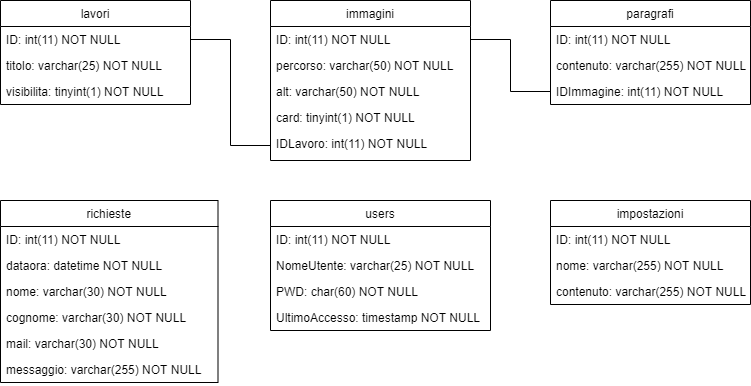
\includegraphics[scale = 0.5]{../latex/images/db.png}\\[1.5cm]
\end{center}

\subsection{Struttura dei contenuti}
dire che c'è lato clienti e lato admin.

\subsubsection{Lato cliente}
qualcosa qualcosa qualcosa qualcosa qualcosa qualcosa qualcosa qualcosa qualcosa qualcosa qualcosa qualcosa qualcosa qualcosa.\\\\
\textbf{Pagine}\\
qualcosa qualcosa qualcosa qualcosa	
	\begin{itemize}
		\item \textbf{Home} \\qualcosa qualcosa
		\item \textbf{Chi siamo}\\qualcosa qualcosa
		\item \textbf{Lavori}\\dire le pagine che lo compongono e cosa contengono
	 	\begin{itemize}
 			\item Matrimoni;\\	qualcosa qualcosa 
	 		\item Lauree;\\	qualcosa qualcosa 
 			\item Funerali;\\	qualcosa qualcosa
 			\item ...; 		 		
	 	\end{itemize}
	 	\item \textbf{Contatti}\\qualcosa qualcosa\\
 	\end{itemize}
\textbf{Parti fondamentali -> troviamoci un sinonimo}\\ 
	qualcosa qualcosa qualcosa
	\begin{itemize}
		\item \textbf{Header}\\qualcosa qualcosa
		\item \textbf{Breadcrumb}\\qualcosa qualcosa
		\item \textbf{Footer}\\qualcosa qualcosa
 	\end{itemize}
 		
\subsubsection{Lato Admin}
- discorso login
- discorso session\\\\
\textbf{Pagine}\\ qualcosa qualcosa qualcosa
	\begin{itemize}
		\item \textbf{Dashboard};\\qualcosa qualcosa
		\item \textbf{Gestione richieste};\\qualcosa qualcosa
		\item \textbf{Gestione categorie};\\dire le pagine che lo compongono e come funziona il tutto
	 	\begin{itemize}
 			\item Aggiungi categoria;\\qualcosa qualcosa
 			\item Modifica categoria;\\qualcosa qualcosa
 			\item Elimina categoria;\\qualcosa qualcosa
	 	\end{itemize}
 	\item \textbf{Gestione utenti}\\qualcosa qualcosa qualcosa
 	\item \textbf{Logout}\\qualcosa qualcosa qualcosa\\
 	\end{itemize}
\textbf{Parti fondamentali -> troviamoci un sinonimo} \\
\begin{itemize}
	\item \textbf{Breadcrumb}\\	qualcosa qualcosa qualcosa
	\item \textbf{Funzionamento PHP}\\	DbConnection ecc.
\end{itemize}